\documentclass[border=4pt]{standalone}
\usepackage{tikz}
\usetikzlibrary{arrows.meta,shapes.multipart}
\begin{document}
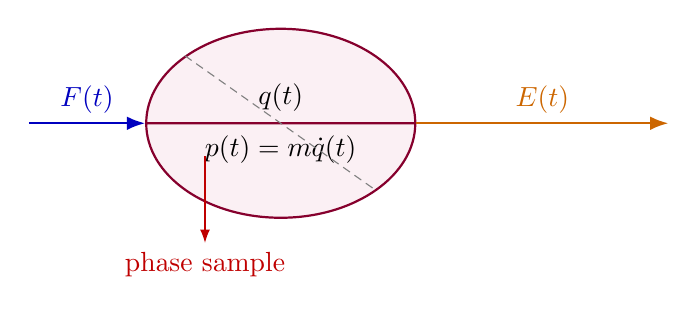
\begin{tikzpicture}[>=Latex]
  \node[ellipse split,draw=purple!70!black,thick,fill=purple!6,
    inner xsep=7pt,inner ysep=4pt,minimum width=30mm,
    minimum height=24mm] (state)
    {$q(t)$\nodepart{lower}$p(t)=m\dot q(t)$};

  \draw[-Latex,thick,blue!75!black] (-32mm,0) --
    node[above] {$F(t)$} (state.west);
  \draw[-Latex,thick,orange!80!black] (state.east) --
    node[above] {$E(t)$} ++(32mm,0);
  \draw[-Latex,red!75!black] (state.lower) -- ++(0,-11mm)
    node[below] {phase sample};
  \draw[gray,densely dashed] (state.north west) -- (state.south east);
\end{tikzpicture}
\end{document}
